\documentclass{article}

\usepackage[margin=1in]{geometry}
\usepackage[colorlinks,linkcolor=blue,filecolor=blue,citecolor=magenta,urlcolor=blue]{hyperref}
\usepackage{bm,amsmath,amsthm,amssymb,multicol,algorithmic,algorithm,enumitem,graphicx,subfigure}
\usepackage{xargs}
\usepackage{stmaryrd}
\usepackage{natbib}
\usepackage{listings}
\usepackage{xcolor}
\usepackage{booktabs} % for professional tables
\definecolor{codegreen}{rgb}{0,0.6,0}
\definecolor{codegray}{rgb}{0.5,0.5,0.5}
\definecolor{codepurple}{rgb}{0.58,0,0.82}
\definecolor{backcolour}{rgb}{0.95,0.95,0.92}

\newtheorem{definition}{Definition}
\newcommand{\algo}{\textsc{eff-EBM}}
\lstdefinestyle{mystyle}{
    backgroundcolor=\color{backcolour},   
    commentstyle=\color{codegreen},
    keywordstyle=\color{magenta},
    numberstyle=\tiny\color{codegray},
    stringstyle=\color{codepurple},
    basicstyle=\ttfamily\footnotesize,
    breakatwhitespace=false,         
    breaklines=true,                 
    captionpos=b,                    
    keepspaces=true,                 
    numbers=left,                    
    numbersep=5pt,                  
    showspaces=false,                
    showstringspaces=false,
    showtabs=false,                  
    tabsize=2
}

\lstset{style=mystyle}


\def\code#1{\texttt{#1}}

\usepackage[linesnumbered,ruled,vlined]{algorithm2e}

\SetCommentSty{mycommfont}
\SetKwInput{KwInput}{Input}                % Set the Input
\SetKwInput{KwOutput}{Output}   


\def\M{\mathcal{M}}
\def\A{\mathcal{A}}
\def\Z{\mathcal{Z}}
\def\S{\mathcal{S}}
\def\D{\mathcal{D}}
\def\R{\mathcal{R}}
\def\P{\mathcal{P}}
\def\K{\mathcal{K}}
\def\E{\mathbb{E}}
\def\F{\mathfrak{F}}
\def\l{\boldsymbol{\ell}}

\newtheorem{Fact}{Fact}
\newtheorem{Lemma}{Lemma}
\newtheorem{Prop}{Proposition}
\newtheorem{Theorem}{Theorem} 
\newtheorem{Def}{Definition}
\newtheorem{Corollary}{Corollary}
\newtheorem{Conjecture}{Conjecture}
\newtheorem{Property}{Property}
\newtheorem{Observation}{Observation}
\newtheorem{Exa}{Example}
\newtheorem{assumption}{H\!\!}
\newtheorem{Remark}{Remark}
\newtheorem*{Lemma*}{Lemma}
\newtheorem*{Theorem*}{Theorem}
\newtheorem*{Corollary*}{Corollary}
 
\newcommand{\eqsp}{\;}
\newcommand{\beq}{\begin{equation}}
\newcommand{\eeq}{\end{equation}}
\newcommand{\eqdef}{\mathrel{\mathop:}=}
\def\EE{\mathbb{E}}
\newcommand{\norm}[1]{\left\Vert #1 \right\Vert}
\newcommand{\pscal}[2]{\left\langle#1\,|\,#2 \right\rangle}
\def\major{\mathsf{M}}
\def\rset{\ensuremath{\mathbb{R}}}





\begin{document}



\title{Weekly Report KARIMI-2021-12-03}


\date{}
\maketitle




My work this week has mainly been towards
\begin{enumerate}
\item Fed-LAMB Arxiv v2
\item AISTATS and ALT Rebuttal 
\item FeaBox paper
\end{enumerate}

\section{Fed-LAMB (more experiments)}
We included the Adaptive Federated Optimization of \citep{reddi2020adaptive} to our several experiments.
Done for single GPU and currently implementing the new baseline in the distributed settings.



\begin{figure}[H]
\vspace{-0.15in}
    \begin{center}
        \mbox{
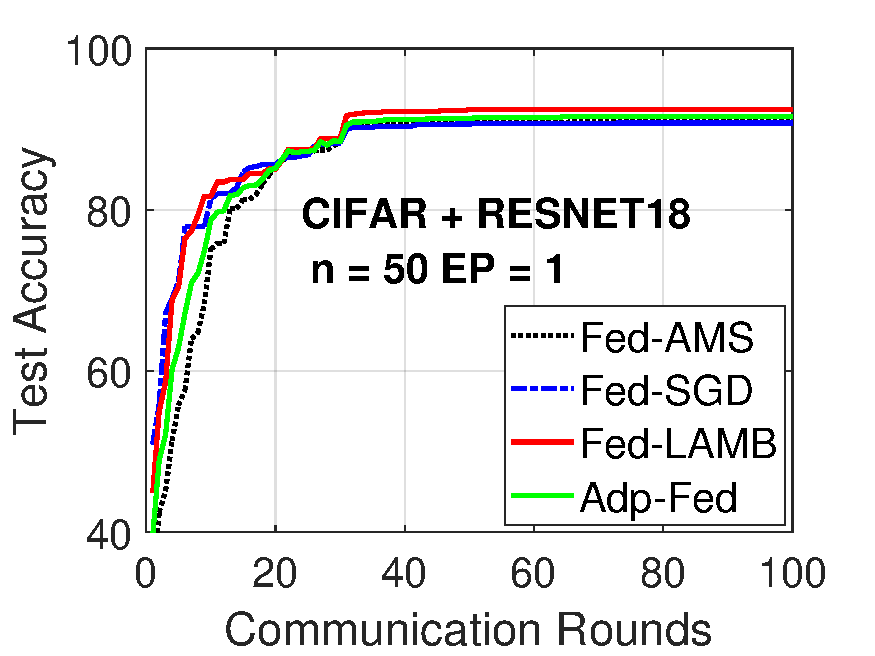
\includegraphics[width=0.4\textwidth]{new_fmnist_mnist_fig/cifar_testerror_resnet18_ep1_client2_iid0_reddi.pdf}
        \hspace{-0.1in}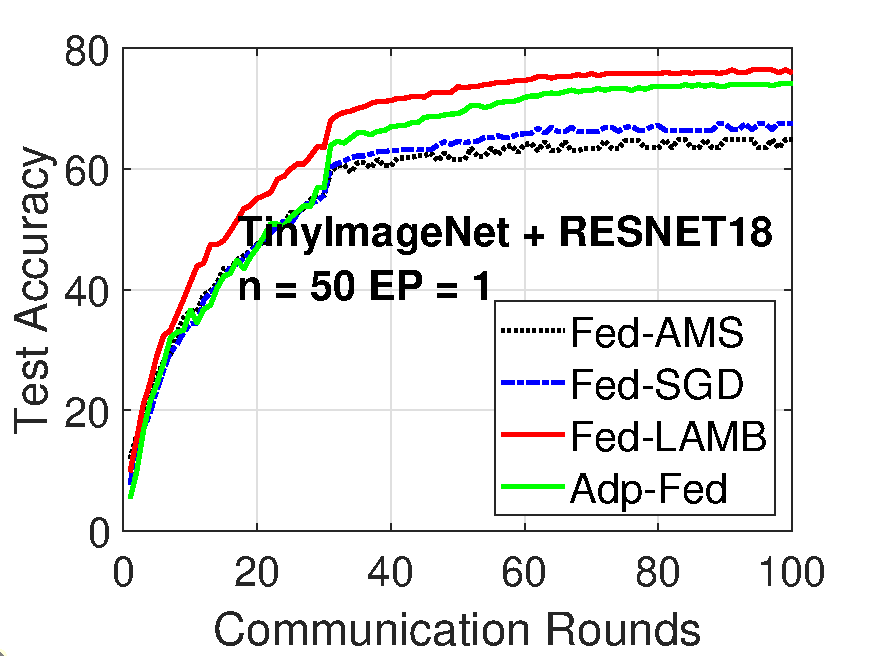
\includegraphics[width=0.4\textwidth]{new_fmnist_mnist_fig/tinyimagenet_testerror_resnet18_ep1_client2_iid0_reddi.pdf}\hspace{-0.1in}
        % \includegraphics[width=0.4\textwidth]{new_figure/tinyimagenet_testerror_resnet18_ep1_client2_iid0.eps}
        }
    \end{center}
    \vspace{-0.2in}
	\caption{\textbf{non-i.i.d. data setting.} Test accuracy on CIFAR-10 + ResNet-18 and TinyImagenet + ResNet-18 with 50 clients.
	}
	\label{fig:noniidresnet18}\vspace{-0.1in}
\end{figure}

\begin{table}[h]
\centering
\caption{Test Accuracy on ResNet-18 Network.}\label{tab:acc}
	\resizebox{0.9\columnwidth}{!}{%
\begin{tabular}{lllll}
\toprule[1pt]
 & Fed-SGD      & Fed-AMS    & Adp-Fed     & \textbf{\algo\ }       \\ \hline
CIFAR-10 & 90.75 $\pm$ 0.48  & 90.93 $\pm$ 0.22 & 91.57 $\pm$ 0.38  & 92.44 $\pm$ 0.53 \\
% TinyImageNet & 79.64 $\pm$ 0.21  & 75.94 $\pm$ 0.83  & 93.50 $\pm$ 0.26 \\
TinyImageNet & 67.58 $\pm$ 0.21  & 64.86 $\pm$ 0.83 & 74.17 $\pm$ 0.43  & 76.00 $\pm$ 0.26 \\
\toprule[1pt]
\end{tabular}
}\vspace{-0.2in}
\end{table}



\section{AISTATS and ALT Rebuttal}
Please refer to the Overleaf projects for the rebuttal




\bibliographystyle{plain}
\bibliography{ref}


\end{document} 